\documentclass[tikz, border=3mm]{standalone}
\usetikzlibrary{positioning, arrows.meta, fit}

\begin{document}
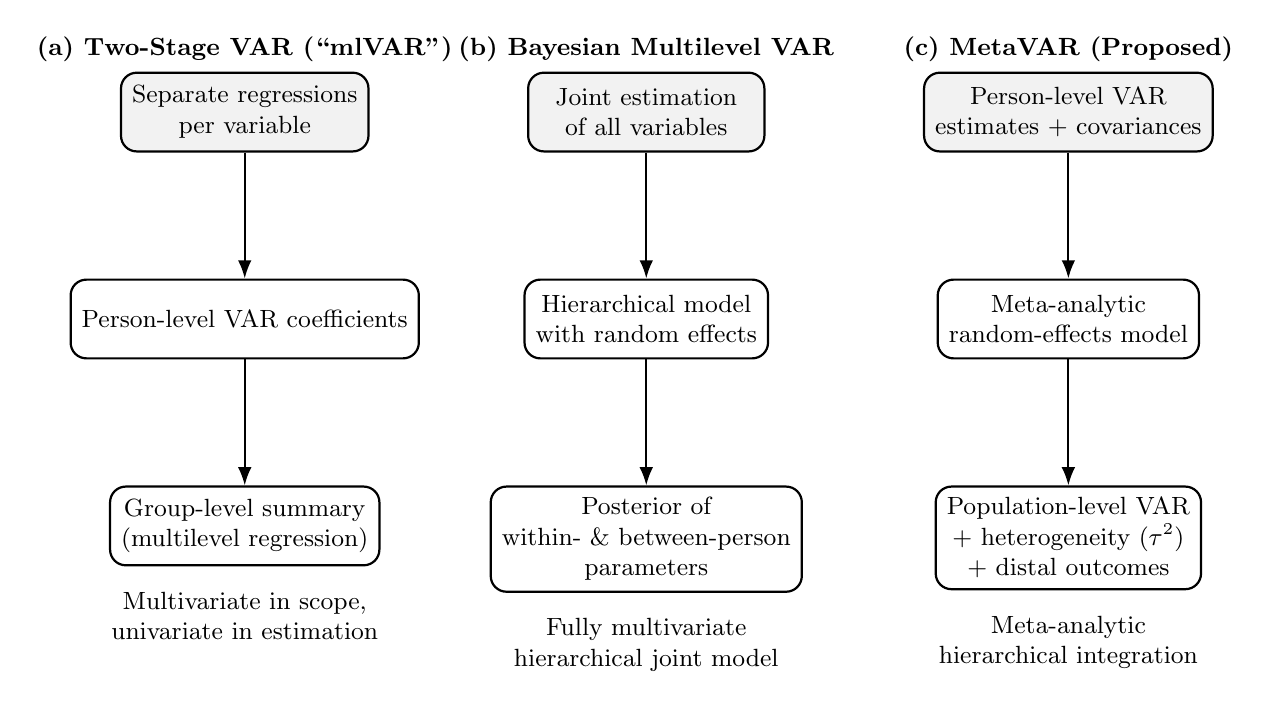
\begin{tikzpicture}[
  node distance = 1.6cm and 2.0cm,
  every node/.style = {align=center, font=\small},
  box/.style = {draw, rounded corners=2mm, thick, inner sep=4pt, minimum width=3cm, minimum height=1cm},
  arrow/.style = {->, thick, >=Latex}
]

% --- mlVAR
\node[box, fill=gray!10, label=above:{\textbf{(a) Two-Stage VAR (``mlVAR'')}}] (mlvar1) {Separate regressions \\ per variable};
\node[box, below=of mlvar1] (mlvar2) {Person-level VAR coefficients};
\node[box, below=of mlvar2] (mlvar3) {Group-level summary \\ (multilevel regression)};
\draw[arrow] (mlvar1) -- (mlvar2);
\draw[arrow] (mlvar2) -- (mlvar3);

% --- Multilevel VAR
\node[box, fill=gray!10, right=of mlvar1, label=above:{\textbf{(b) Bayesian Multilevel VAR}}] (bml1) {Joint estimation \\ of all variables};
\node[box, below=of bml1] (bml2) {Hierarchical model \\ with random effects};
\node[box, below=of bml2] (bml3) {Posterior of \\ within- \& between-person \\ parameters};
\draw[arrow] (bml1) -- (bml2);
\draw[arrow] (bml2) -- (bml3);

% --- MetaVAR
\node[box, fill=gray!10, right=of bml1, label=above:{\textbf{(c) MetaVAR (Proposed)}}] (meta1) {Person-level VAR \\ estimates + covariances};
\node[box, below=of meta1] (meta2) {Meta-analytic \\ random-effects model};
\node[box, below=of meta2] (meta3) {Population-level VAR \\ + heterogeneity (\(\tau^2\)) \\ + distal outcomes};
\draw[arrow] (meta1) -- (meta2);
\draw[arrow] (meta2) -- (meta3);

% --- Titles
\node[below=0.2cm of mlvar3] {Multivariate in scope, \\ univariate in estimation};
\node[below=0.2cm of bml3] {Fully multivariate \\ hierarchical joint model};
\node[below=0.2cm of meta3] {Meta-analytic \\ hierarchical integration};

\end{tikzpicture}
\end{document}
